\chapter{Huracán Katrina} \label{cap0b}
%\addcontentsline{toc}{chapter}{Huracán Katrina}

\begin{flushright}
\begin{minipage}{7.85cm}
    {\em Los huracanes han matado más gente en el mundo entero en los últimos
    50 años que ningún otro desastre natural.} \\ Kerry Emanuel
\end{minipage}
\end{flushright}

\vspace*{5mm}

\section{Introducción}

El huracán Katrina fue uno de los ciclones tropicales más mortíferos,
destructivos y costosos que haya impactado a Estados Unidos en décadas. Katrina
formó parte de la Temporada de huracanes en el Atlántico de 2005. Fue la tercera
tormenta más poderosa de la temporada.

\begin{figure}[H]
 \centering
 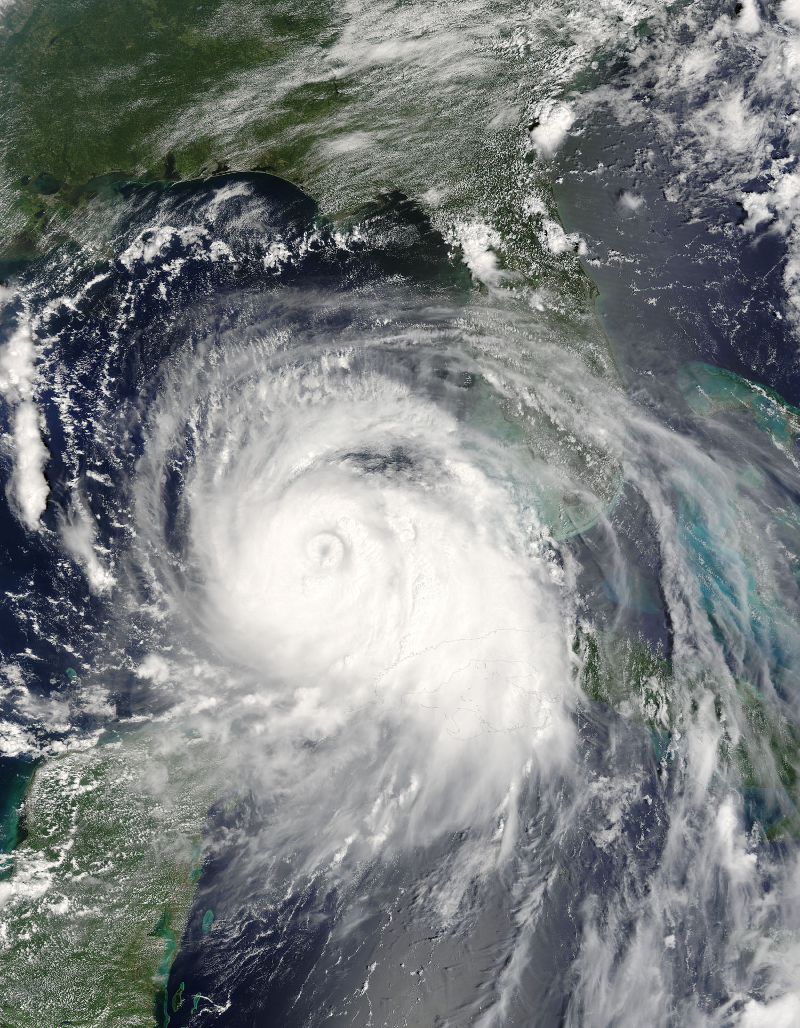
\includegraphics[height=50mm]{figuras/cap0/hurricane.png}
 \caption{Huracán Katrina visto desde el espacio}
\end{figure}

Fue un gran ciclón tropical que azotó el sur y el centro de los Estados Unidos
en agosto de 2005. Produjo grandes destrozos en Florida, Bahamas, Luisiana y
Misisipi, incluyendo cuantiosos daños materiales y graves inundaciones.

\begin{figure}[H]
 \centering
 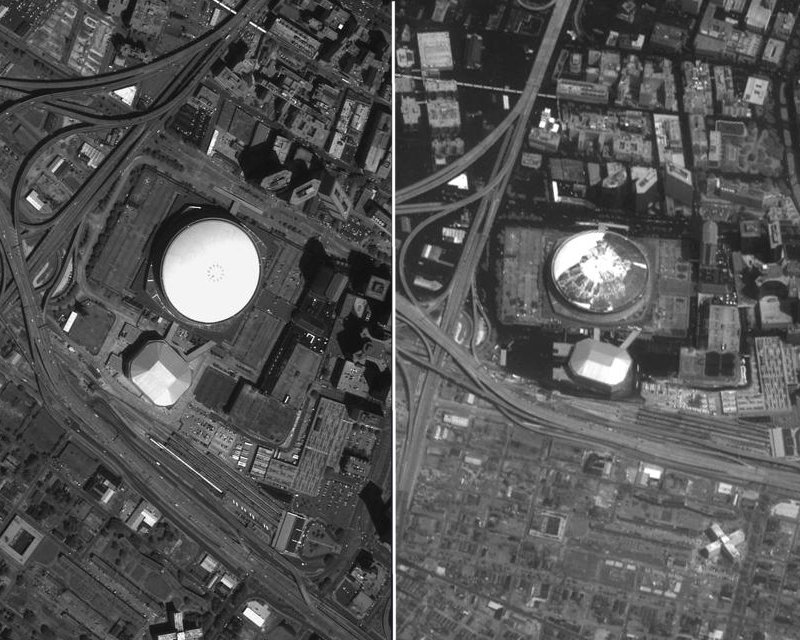
\includegraphics[width=120mm]{figuras/cap0/before_after.png}
 \caption{Daños producidos por el huracán al {\em Superdome}}
\end{figure}

Tocó tierra en la costa de Luisiana el 29 de agosto convertido en un huracán
categoría 4\cite{DeLozier}, y a pesar de que en el último momento se desvió
ligeramente de su ruta, que originalmente atravesaba directamente la ciudad de
Nueva Orleans, se produjo una gran devastación en la misma y en zonas cercanas.
Por los daños producidos, se convirtió en uno de los huracanes más devastadores
en Estados Unidos en la historia reciente.

Se estima que el Katrina causó daños materiales por 75 mil millones de dólares
estadounidenses, convirtiéndose en el huracán más costoso en la historia de los
Estados Unidos; la tormenta causó la muerte a 1833 personas, convirtiéndose en
el huracán más mortífero de Estados Unidos desde el Huracán Okeechobee de
1928\cite{Knabb05}.

\section{Efectos en Nueva Orleans}

El 2 de septiembre de 2005 el 85\% de la ciudad de Nueva Orleans estaba bajo el
agua, donde en algunas zonas llegó a 7 m de profundidad. Durante un tiempo, la
ciudad estuvo inhabitable. Todos los servicios públicos estaban suspendidos y no
era posible utilizar la infraestructura física debido a la gran cantidad de
agua. Además estaba en crisis de orden público debido al violento saqueo
generalizado que se presenta por la falta de alimentos y seguridad. El
{\em Superdome}, principal refugio "de última hora" tuvo que ser evacuado
debido al deterioro de las condiciones de vida en su interior (daño a los
generadores, falta de aire acondicionado e interrupción del servicio de
entrega de agua).

\begin{figure}[H]
 \centering
 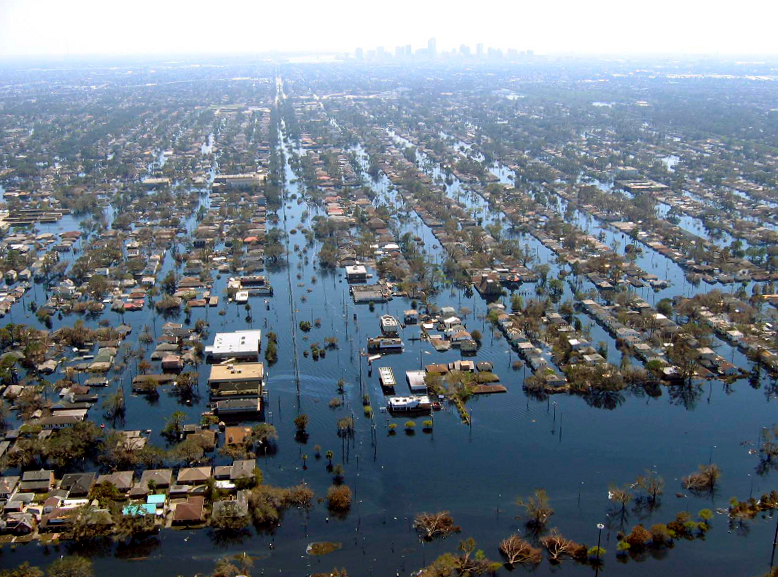
\includegraphics[width=130mm]{figuras/cap0/flood.png}
 \caption{La ciudad de Nueva Orleans inundada}
\end{figure}

Durante los días anteriores se generalizó el vandalismo y la escasez de
alimentos, vivienda y agua produjo un desorden civil de grandes proporciones. La
tarde del 1 de septiembre, la oficina del alcalde pidió ayuda urgente para
controlar la situación que había alcanzado niveles desmedidos. Durante varios
días estuvo vigente la ley marcial, el uso de la fuerza contra el saqueo y la
recomendación urgente de abandonar la ciudad a través de la conexión con
Crescent City, o en su defecto buscar refugio en pisos más altos. La rotura de
una sección del dique hizo que el nivel de agua aumentase en vez de disminuir, y
los esfuerzos para reconstruirlo temporalmente arrojando bolsas de arena desde
helicópteros no resultaron efectivos. En la tarde del 30 de agosto, y en
atención a la imposibilidad de restaurar el aislamiento con el lago
Pontchartrain, y al empeoramiento de las condiciones de vida en los albergues,
la gobernadora de Luisiana, Kathleen Blanco, ordenó la evacuación de todos los
residentes de Nueva Orleans\cite{DeLozier}.

\begin{figure}[H]
 \centering
 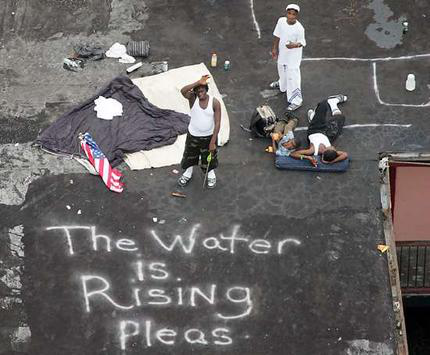
\includegraphics[width=80mm]{figuras/cap0/help.png}
 \caption{Afectados solicitando ayuda en Nueva Orleans}
\end{figure}

\section{Estudios e Información sobre el Desastre}

Como el huracán afectó a Estados Unidos, país desarrollado y con grandes
recursos, hay mucha información disponible. Información meteorológica sobre la
evolución y desarrollo del huracán\cite{Blake07}, e información sobre las
pérdidas humanas y materiales\cite{Knabb05}\cite{Gabe05}, así como informes
sobre la actuación de las fuerzas de seguridad y emergencias del
estado\cite{DeLozier}. También es posible encontrar información sobre los
evacuados\cite{Groen08}, estudios demográficos\cite{McCarthy06},
encuestas\cite{Washington05}, etc.

Aparte de todos estos estudios, también es muy importante contar con
información geográfica del terreno afectado. Afortunadamente, y una vez más,
dado que se trata de Estados Unidos, contamos con varias fuentes de información.

La U.S. Geological Survey (USGS\footnote{\url{http://www.usgs.gov/}}) es una
institución gubernamental dedicada al estudio biológico, geológico, geográfico y
geoespacial de Estados Unidos. Entre otras muchas funciones, mantiene una base
de datos de información sobre la altura del terreno, la National Elevation
Dataset (NED\footnote{\url{http://ned.usgs.gov/}}. Dicha base de datos contiene
información de múltiples fuentes, incluso proveniente de la Shuttle Radar
Topography Mission (SRTM\footnote{\url{http://www2.jpl.nasa.gov/srtm/}})
desarrollada por la National Aeronautics and Space Administration (NASA). Estos
datos alcanzan en algunas zonas -como es el caso de Nueva Orleans- la precisión
de $^1/_9$ de segundo de arco (aproximadamente 3 metros).

Existen también servicios de información con los datos relativos a la
organización de las ciudades: calles, parques, etc. Un servicio que proporciona
información de calidad, y de acceso libre, sobre Nueva Orleans es Open Street
Maps (OSM\footnote{\url{http://www.openstreetmap.org/}}.

La forma de acceder y procesar estos datos se presenta en capítulos posteriores.

%%% Local Variables:
%%% mode: latex
%%% TeX-master: "../dissim"
%%% End: